\documentclass[10pt]{beamer}

\usetheme[progressbar=frametitle]{metropolis}
\usepackage{appendixnumberbeamer}

\usepackage[ngerman]{babel}
\usepackage[latin1]{inputenc}

\usepackage{booktabs}
\usepackage[scale=2]{ccicons}

\usepackage[center]{caption}

\usepackage{pgfplots}
\usepgfplotslibrary{dateplot}

\usepackage{xspace}
\newcommand{\themename}{\textbf{\textsc{metropolis}}\xspace}

\title{R�ckgekoppelte neuronale Netze}
\subtitle{Eine Einf�hrung}
% \date{\today}
\date{}
\author{Konstantin Tieber}
\institute{webfactory GmbH}
% \titlegraphic{\hfill\includegraphics[height=1.5cm]{logo.pdf}}

\begin{document}

\maketitle

%\begin{frame}{Inhalt}
%  \setbeamertemplate{section in toc}[sections numbered]
%  \tableofcontents[hideallsubsections]
%\end{frame}

%\section{Einf�hrung in r�ckgekoppelte Netze}

\begin{frame}{Warum r�ckgekoppelte neuronale Netze?}
	\begin{itemize}
		\item eignen sich sehr gut zur Verarbeitung von Daten, die eine Sequenz darstellen.
		\item Anwendungsbereiche\begin{itemize}
			\item Sprachverarbeitung %Ton menschlicher Sprache
			\item Audioverarbeitung % nur Ton bzw. Musik
			\item Videoverarbeitung
			\item Sprachmodellierung %t ext
		\end{itemize}
		%HIER DEMO Sprachmodellierung
	\end{itemize}
\end{frame}

\begin{frame}{Phase Eins}
	\begin{figure}
		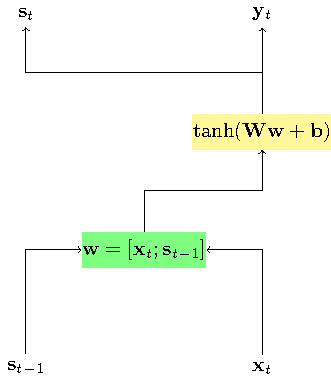
\includegraphics[scale=1]{../bilder_intro/recurrent_cell.pdf}
		\caption*{Einfache r�ckgekoppelte Zelle}
		% kleinBuchstaben = Vektoren, gro�Buchstaben: Matrizen
		% simple r�ckgekoppelte neuronale Netze funktionieren deswegen nicht
		% Buchstabe x kommt rein
		% verbinde input und speicher Vektor
		% kombiniere Vektoren durch Matrizen-Multiplikation
		% hyperbolischer Tangens skaliert die Vektoren (Werte zwischen 0 und 1)
		% aktualisiere den Speicher mit neuem Vektor aus Neuron (Speicher f�r n�chsten Zeitschritt)
		% y ist die Wahrscheinlichkeitswerte von Buchstaben unseres Outputs
	\end{figure}
\end{frame}

\begin{frame}{Probleme}
	\begin{itemize}
		\item es wird alles gespeichert und nichts vergessen
		\item verschwindender Gradient % unbesiegbar?
		\item explodierender Gradient % clipping Funktion, um gro�e Zahlen "abzurasieren"
	\end{itemize}
\end{frame}

\begin{frame}{L�sung}
	\begin{figure}
		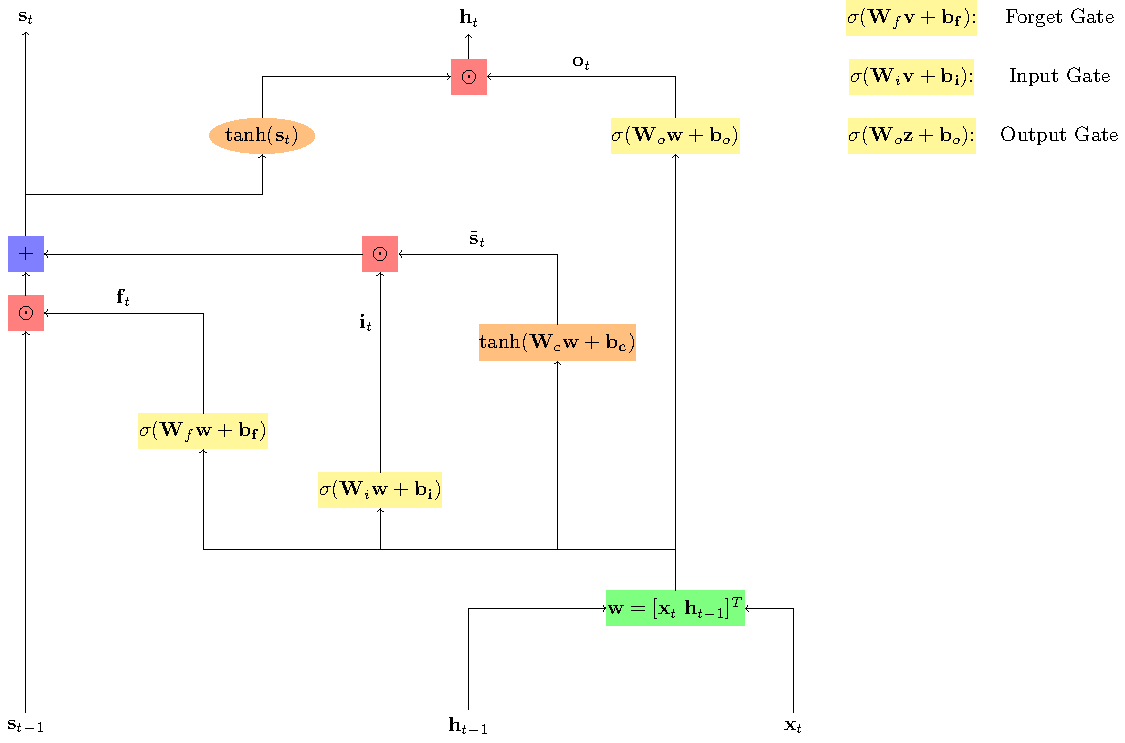
\includegraphics[scale=0.5]{../bilder_intro/nop_lstm.pdf}
		\caption*{Schematische Darstellung einer Long Short Term Memory Zelle}
		% s (speicherlinie) ist ein Log vorhergegangener Operationen
		% h vorheriger Output und x neuer Input kommen rein, werden kombiniert
		% f beinhaltet was ich vergessen m�chte
		% i beinhaltet was ich speichern m�chte (Input Gate Ausgang) 1 = speichern, 0 = nicht speichern
		% o beinhaltet was raus darf
		% f, i und o sind Ausgangswerte einer sigmoiden Funktion (Werte zwischen 0 und 1)
		% die sigmiod Funktionen ergeben eine Zahl zwischen 0 und 1, welche bestimmt wie viel vom Vektor "passieren" darf
		% hyperbolische Tangens sind die echten Daten (-1 bis 1) und Sigmoide Funktionen sind Tore
	\end{figure}
\end{frame}

\begin{frame}{Problem}
	\begin{itemize}
		\item Wir bestimmen, was vergessen, gespeichert und ausgegeben werden soll, ohne den Inhalt des Speichers zu kennen.
	\end{itemize}
\end{frame}

\begin{frame}{L�sung}
	\begin{figure}
		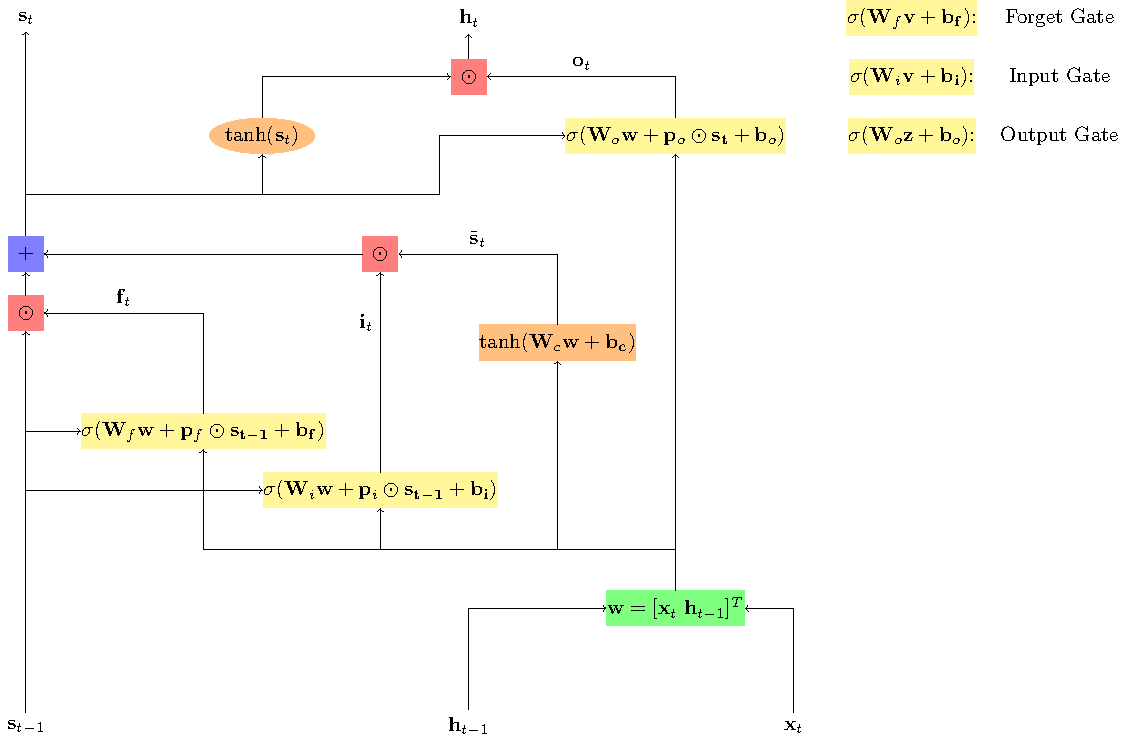
\includegraphics[scale=0.5]{../bilder_intro/lstm.pdf}
		\caption*{Schematische Darstellung einer Long Short Term Memory Zelle\\mit Kuckl�chern}
		% empirische Beobachtungen belegen, dass LSTMs mit Kuckl�chern bessere Ergebnisse erzielen
	\end{figure}
\end{frame}

\begin{frame}{Zusammenfassung}
	\begin{itemize}
		\item tbd
	\end{itemize}
\end{frame}

\begin{frame}{Leichte Literatur}
	\begin{itemize}
		\item \href{http://colah.github.io/posts/2015-08-Understanding-LSTMs/}{http://colah.github.io/posts/2015-08-Understanding-LSTMs/}
		\item \href{http://karpathy.github.io/2015/05/21/rnn-effectiveness/}{http://karpathy.github.io/2015/05/21/rnn-effectiveness/}
	\end{itemize}
\end{frame}

\end{document}
